\documentclass[a4paper,14px]{article}
\usepackage[left=2cm,right=2cm]{geometry}
\usepackage{graphicx}
\usepackage{float}

\title{``SITIO WEB PARA LA GESTIÓN Y PROMOCIÓN DE CONGRESOS INTERNACIONALES EN INSTITUCIONES DE EDUCACIÓN SUPERIOR''}

\author{Ing. Stalin Francis Quinde.\\ Ing. Baster Estupiñan. \\ Ing. Diego Hurtado Sotalin.\\  Nayade Caridad Reyes Palau. }
\begin{document}
\maketitle

\section{Antecedente}
\label{sec:antecedente}
La Facultad de Ingenierías pedagogía de la Universidad Técnica Luis Vargas Torres (UTLVTE), organizó un congreso internacional llamado \textbf{``MIRADAS Y TENDENCIAS  DE LAS CIENCIAS INGENIERILES (MTCI) UTLVTE-2022''}, para lo cual necesitaba una plataforma web que le permitiera gestionar y difundir la información que  fue generada desde el momento de su concepción, hasta la culminación que se da con la presentación de las ponencias nacionales e internacionales.\\

Para lograr este objetivo tres docentes de la Facultad se apoyo en la carrera de Tecnología de la Información de la UTLVTE, donde docentes con experiencia en desarrollo web evaluaron varias alternativas a fin de poder aplicar la mejor solución en función de las necesidad y limitaciones que se presentaron en el levantamiento de la información.\\

De todas las soluciones ya existentes, ninguna se ajustaba de forma precisa a las restricciones de este evento, las cuales eran  gran variedad de recursos multimedia, fácil de navegar desde dispositivos móviles y  más que todo bajo presupuesto para su desarrollo por ser evento sin fines de lucro pero de gran nivel académico; unas alternativas resultaron complejas de aprender y con muchas limitación en su versión libre; otras, muy buenas por cierto, resultaban costosas para poder ser utilizadas.\\

Se decidió que al contar con docentes con conocimientos y experiencias en el desarrollo web,  se podía crear un  sitio web propio, para poder  cumplir con el propósito a pesar de las restricciones antes indiadas.\\

Así nace el  ``Sitio Web para la gestión y promoción de congresos internacionales en instituciones de educación superior'' desarrollado por docentes de la UTLTE , el cual se constituye en un  conjunto de programas que utilizan las  herramientas,  html,css,javascrip, php, y mysql; y que se alojan al lado del Servidor Web para poder guardar, recuperar y mostrar la información multimedia de una forma sencilla, sistemática y ordenada desde y en cualquier parte del mundo a través de internet.\\

\section{Descripción de la arquitectura resumida}
\label{sec:descripcion-de-la}


En la gráfica siguiente se muestra de forma resumida como funciona el sitio, los programas estaran alojados en un servidor que se comunicara vía protocolo \textbf{http} con programas navegadoras que se encuentras instaladas en máquina situadas en cualquier parte del mundo, desde donde el usuario puede soluccitar(request) información información que ha sido guardada. \\


\begin{figure}[H]
  \centering
  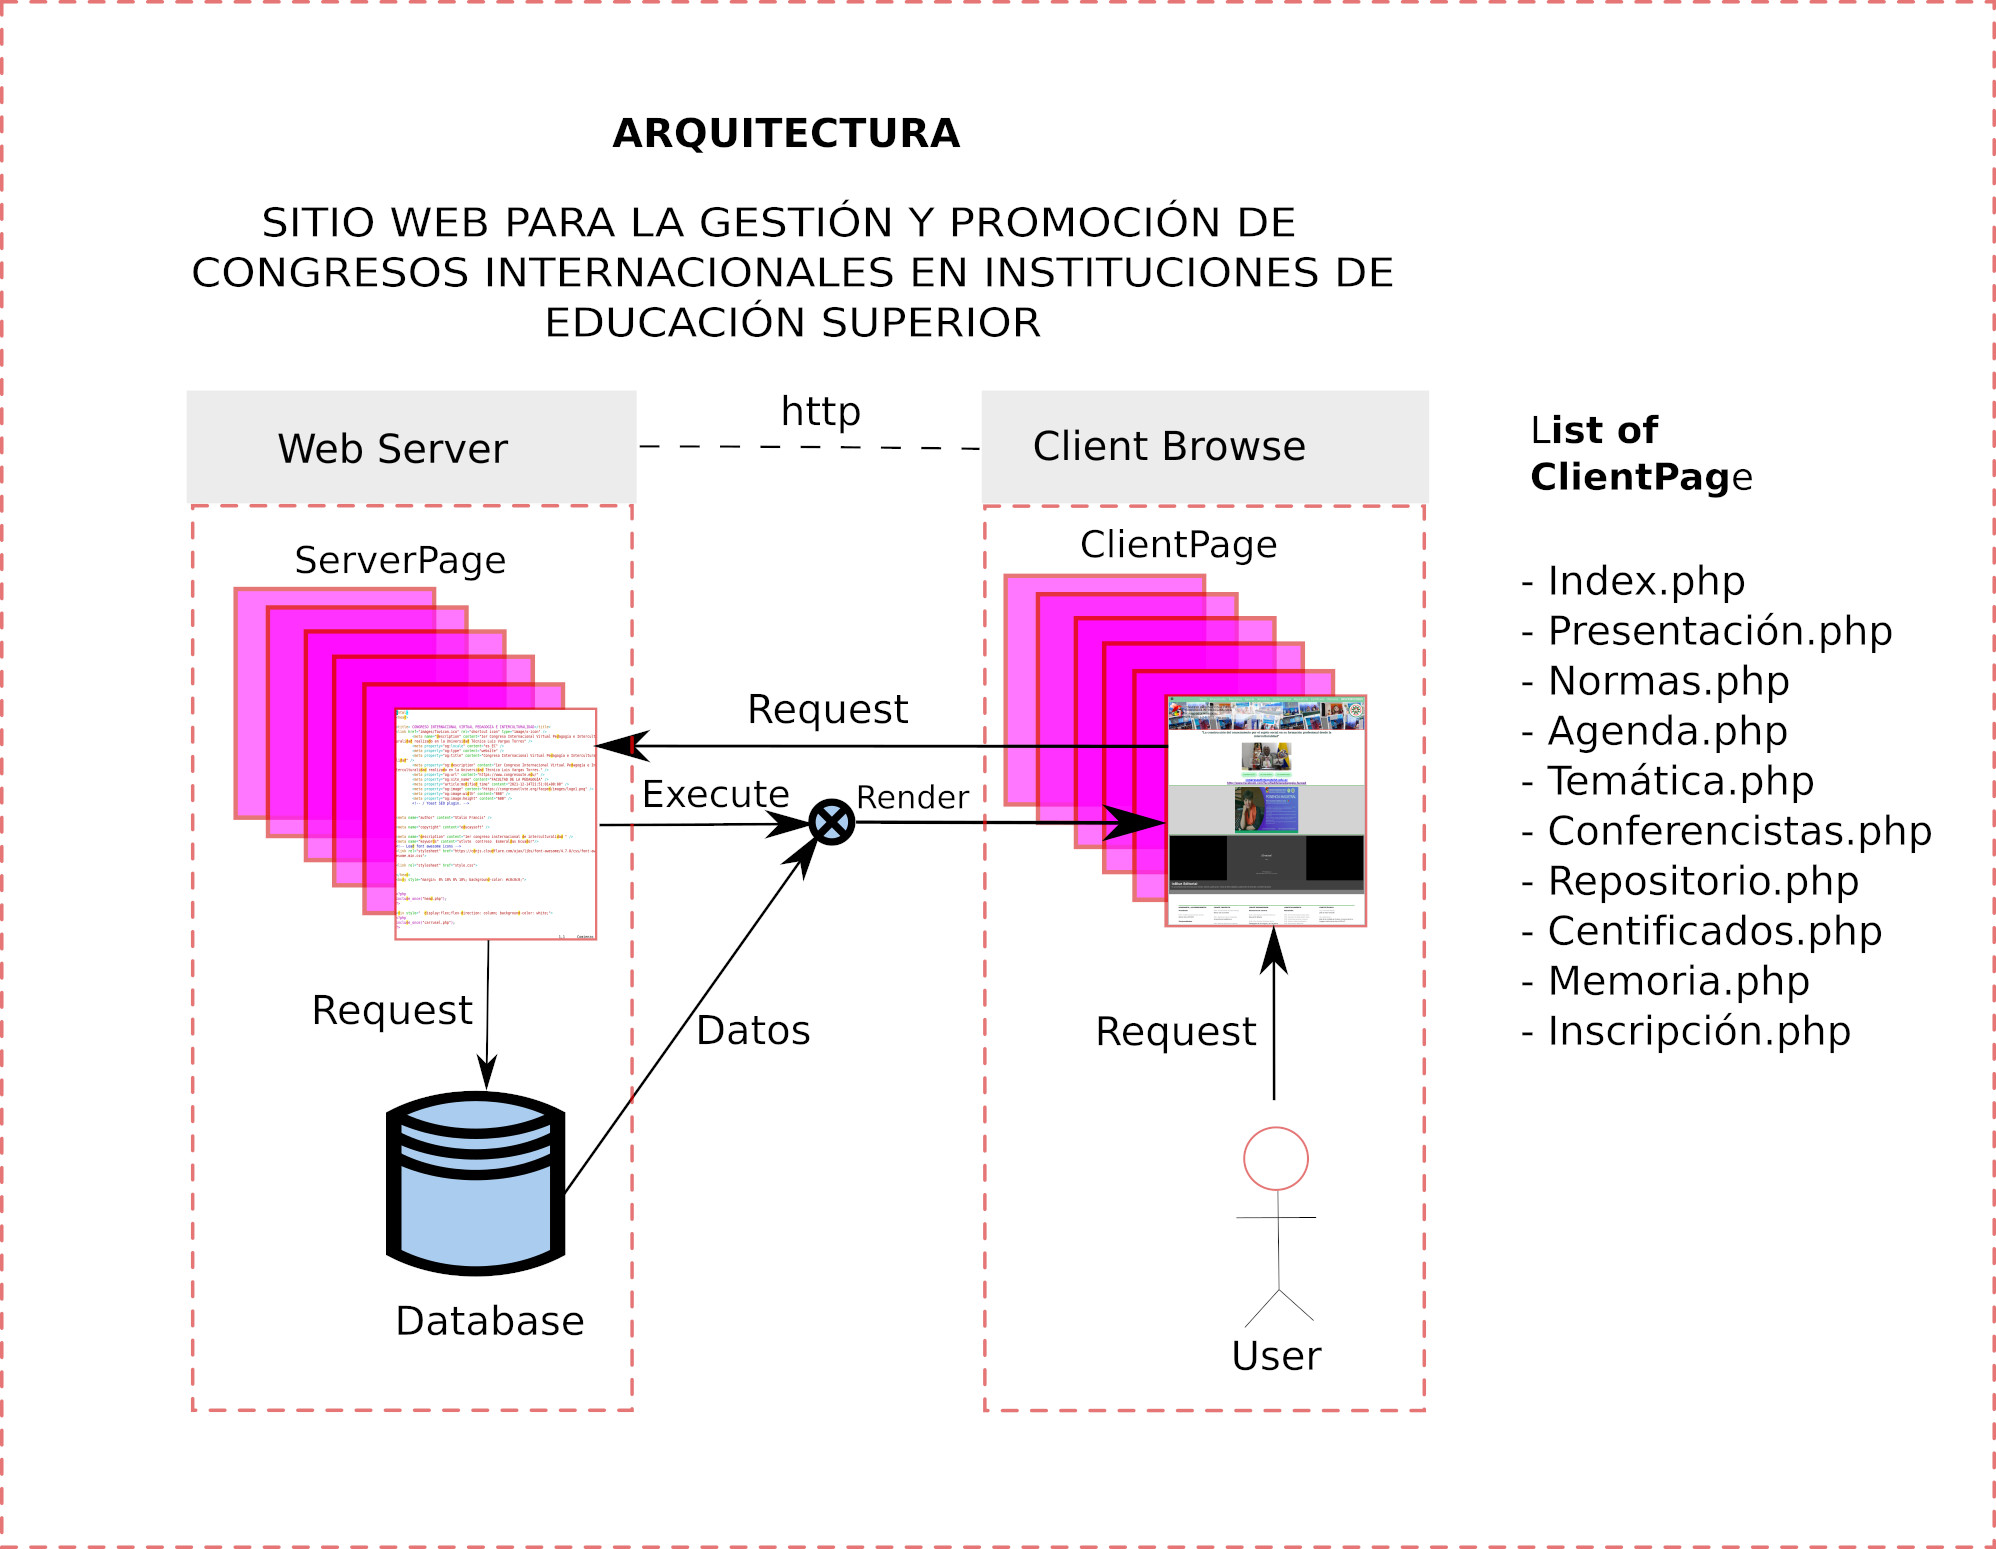
\includegraphics[scale=0.3]{congresoweb.jpg}
  \caption{Arquitectura resumida}
  \label{fig:arquitectura}
\end{figure}


\newpage
\subsection{Página principal}
\label{sec:pagina-principal}

Esta es la página principal del sitio web donde se pone a disposición la información más relevante.



\begin{figure}[H]
  \centering
  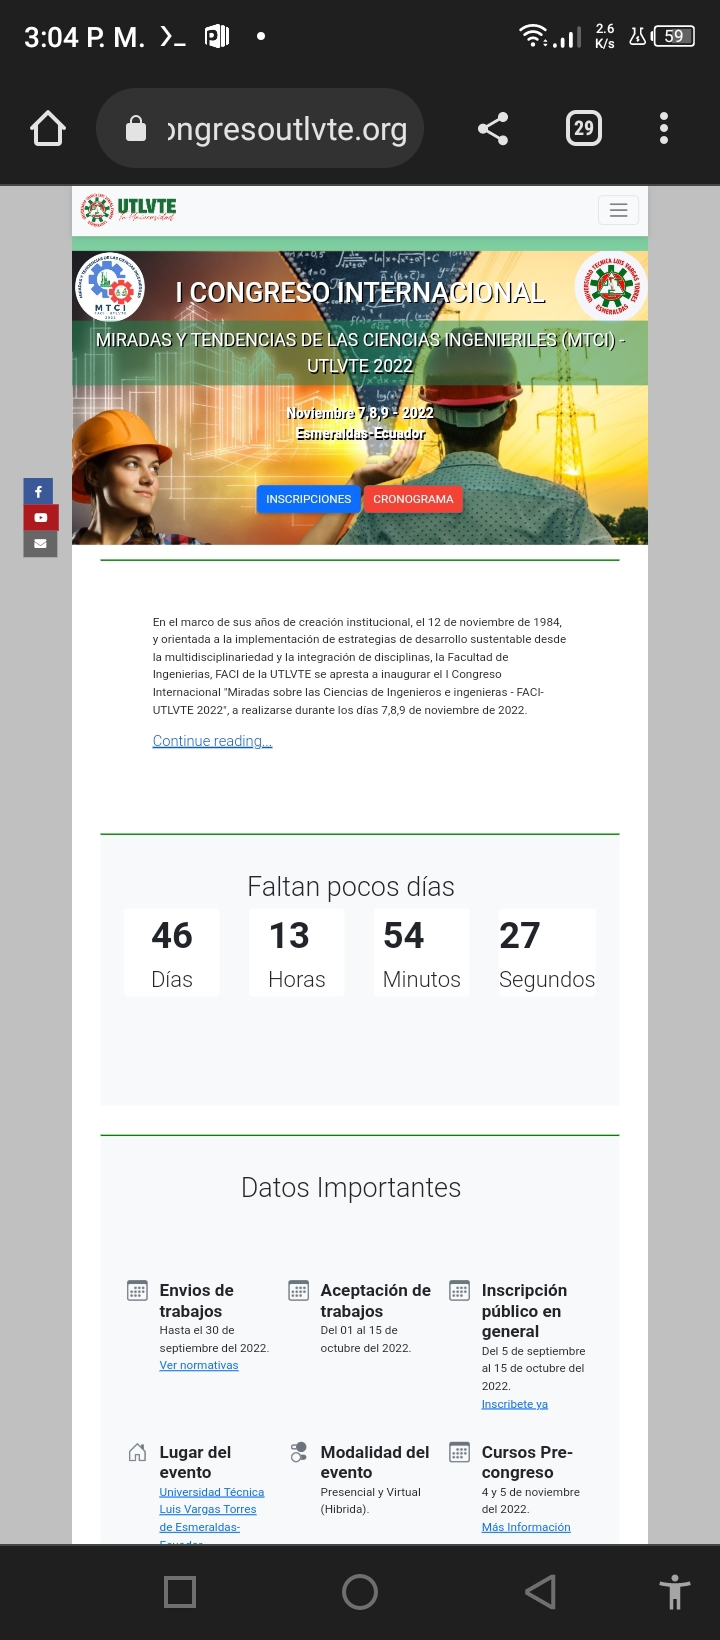
\includegraphics[scale=0.6]{index.jpg}
  \caption{index.php }
  \label{fig:arquitectura}
\end{figure}




\newpage
\subsection{Página bienvenida }
\label{sec:pagina-principal}

Esta es la página donde se da la bienvenida al congreso.


\begin{figure}[H]
  \centering
  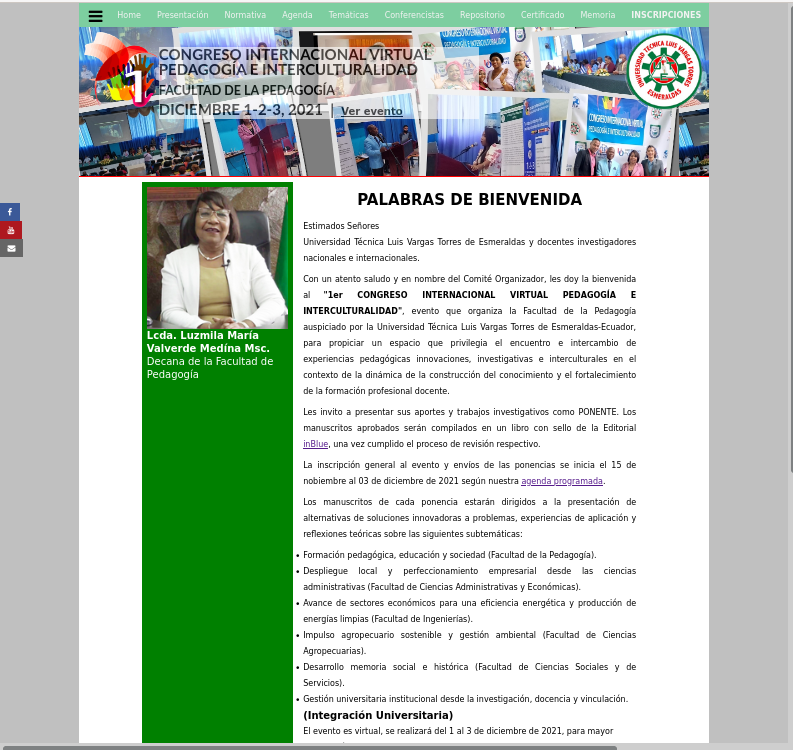
\includegraphics[scale=0.6]{presentacion.png}
  \caption{Presentación}
  \label{fig:arquitectura}
\end{figure}

\newpage
\subsection{Página de normas de presentación }
\label{sec:pagina-principal}

Esta es la página  donde se muestra las normas a seguir para que los ponentes entreguen sus información.



\begin{figure}[H]
  \centering
  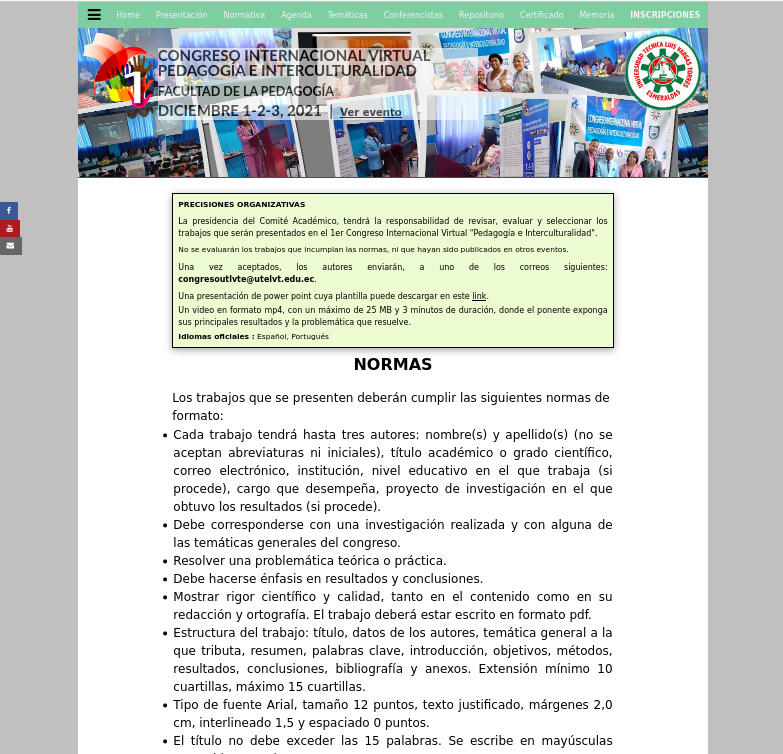
\includegraphics[scale=0.6]{normativas.png}
  \caption{Normativas}
  \label{fig:arquitectura}
\end{figure}


\newpage
\subsection{Página de agenda }
\label{sec:pagina-principal}

En esta página se muestra todo el cronograma de las actividades a realizar mientras dure el congreso, también se da la opción de descargarlo en un archivo pdf.



\begin{figure}[H]
  \centering
  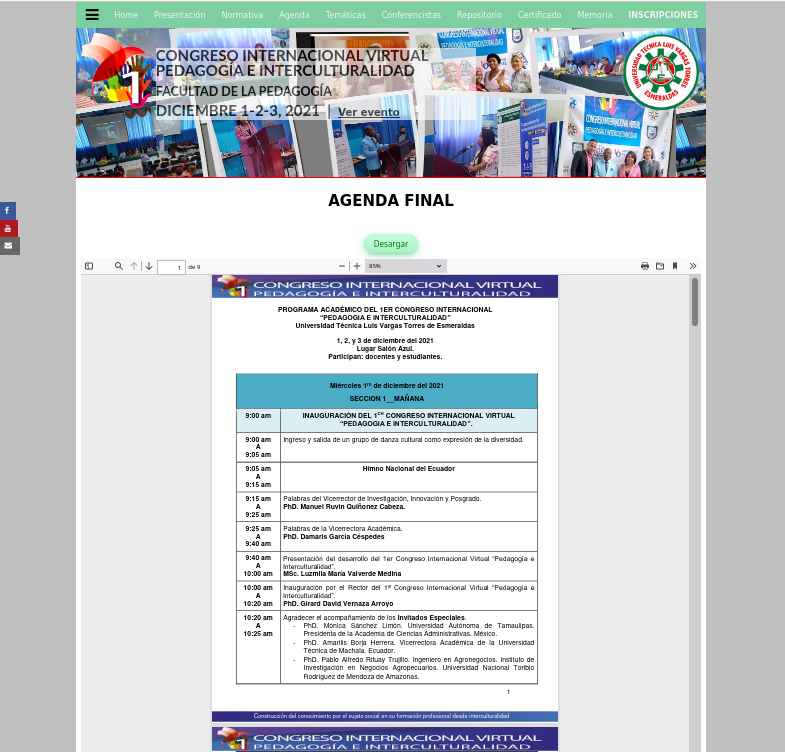
\includegraphics[scale=0.6]{agenda.png}
  \caption{Agenda}
  \label{fig:arquitectura}
\end{figure}


\newpage
\subsection{Página de temáticas }
\label{sec:pagina-principal}

La conferencias preparadas por los ponentes debe realizarse en función de ejes temáticos definidos por la unidad de investigación de la Universidad auspiciantes.


\begin{figure}[H]
  \centering
  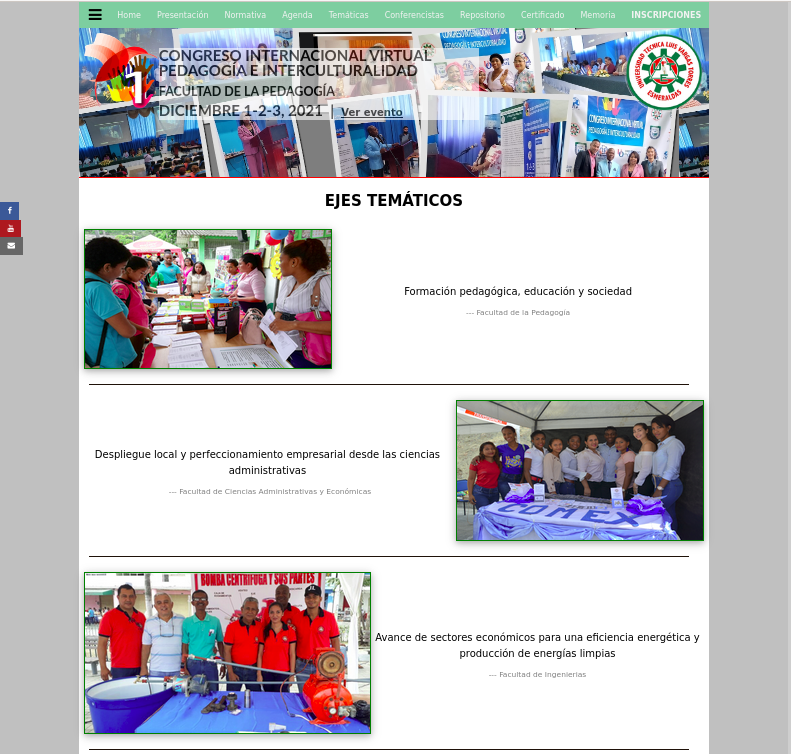
\includegraphics[scale=0.6]{tematicas.png}
  \caption{Temátias}
  \label{fig:arquitectura}
\end{figure}


\newpage
\subsection{Página de confenebienvenida }
\label{sec:pagina-principal}

Los temas y los conferencistas son mostrados en esta página, al lada de cada conferencista tambien se muestra la diapositiva y el video de su ponencia pre-alaborada al menos por el problema de covid-19.



\begin{figure}[H]
  \centering
  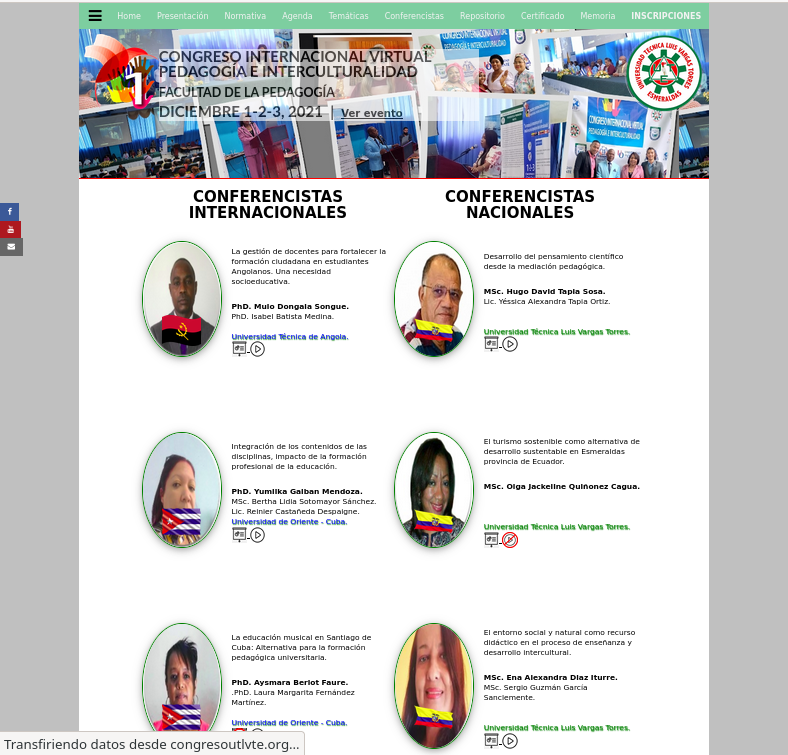
\includegraphics[scale=0.6]{conferencistas.png}
  \caption{Conferencistas}
  \label{fig:arquitectura}
\end{figure}


\newpage
\subsection{Página de repositorio. }
\label{sec:pagina-principal}

El evento debe generar documento y libros por lo que en esta espacio





\begin{figure}[H]
  \centering
  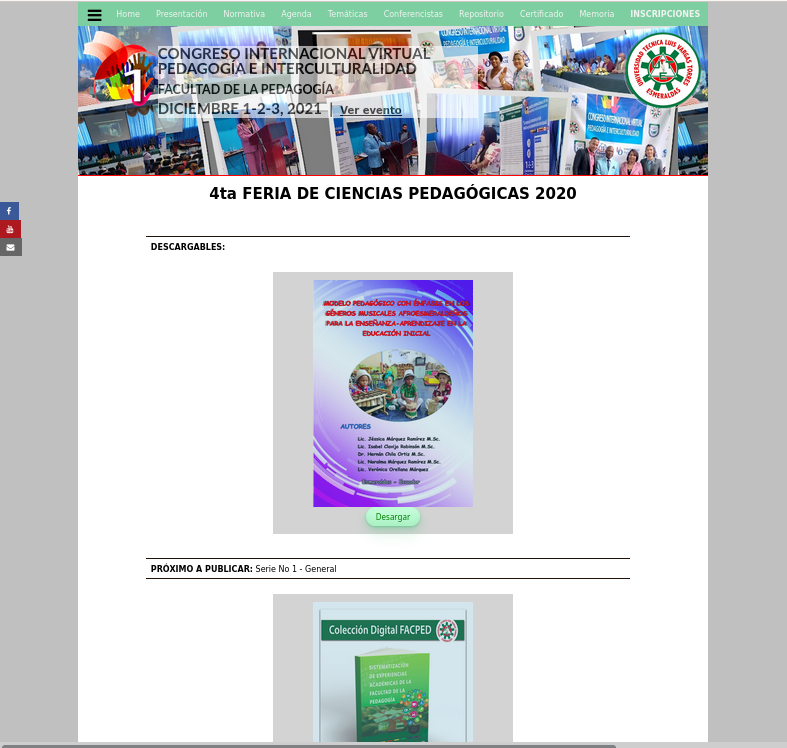
\includegraphics[scale=0.6]{repositorio.png}
  \caption{Repositorio}
  \label{fig:arquitectura}
\end{figure}

\newpage
\subsection{Página para acceder a certificados }
\label{sec:pagina-principal}

Esta página se vincula con otro sistema informático que maneja un base de datos donde se puede acceder a todos los certificados emitidos durante el congreso a los participantes
.



\begin{figure}[H]
  \centering
  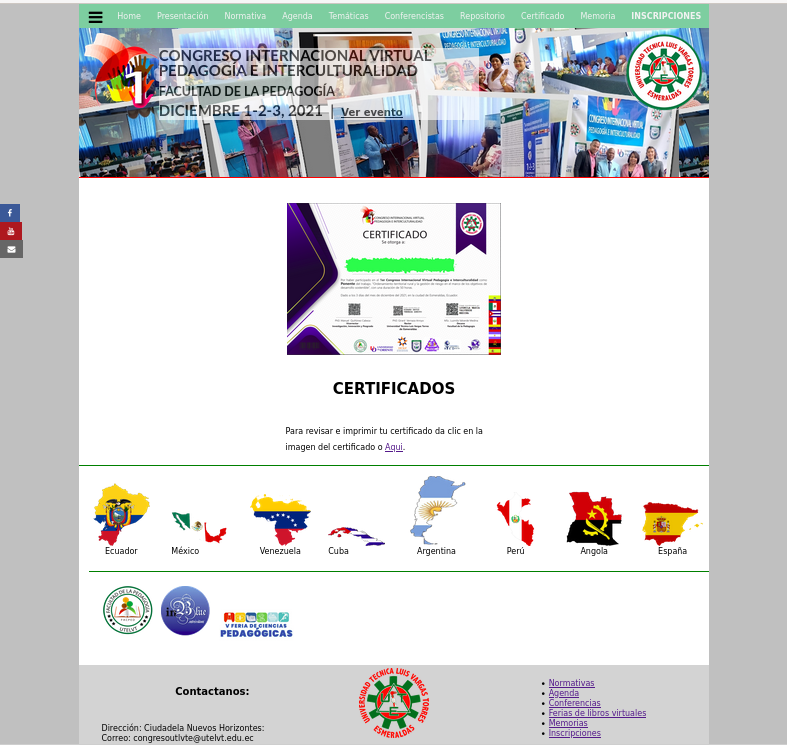
\includegraphics[scale=0.6]{certificado.png}
  \caption{certificadoa}
  \label{fig:arquitectura}
\end{figure}


\newpage
\subsection{Página para mostrar la memora generada}
\label{sec:pagina-principal}

En esta página web se presenta todo los afíches generados y difundidos para dar a conocer el evento del congreso a realizarse..


\begin{figure}[H]
  \centering
  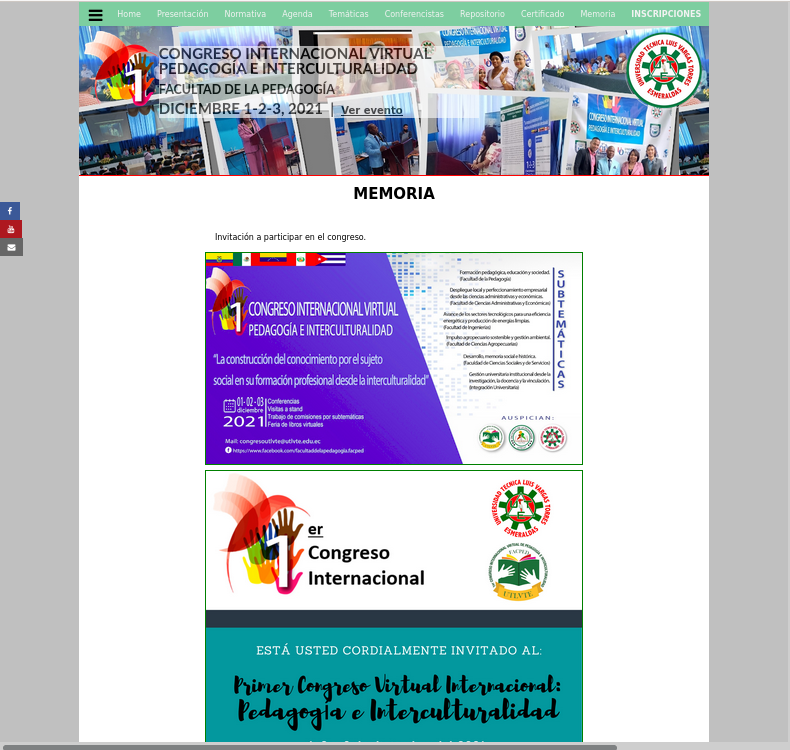
\includegraphics[scale=0.6]{memoria.png}
  \caption{Memoria}
  \label{fig:arquitectura}
\end{figure}

\newpage
\subsection{Página para inscripciones }
\label{sec:pagina-principal}

Esta página web permite acceder a un registro o formulario donde las personas que quieren participar en el congreso puedan dejar sus datos personales, datos que serán utilizados para generar los certificados respectivos.



\begin{figure}[H]
  \centering
  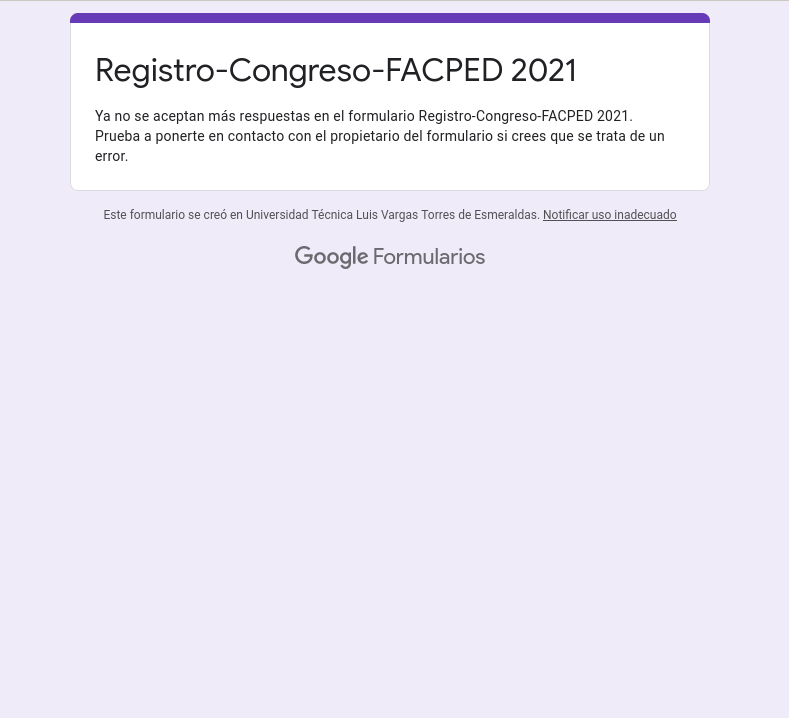
\includegraphics[scale=0.6]{inscripcion.png}
  \caption{Inscripcciones}
  \label{fig:arquitectura}
\end{figure}





\end{document}

%%% Local Variables:
%%% mode: latex
%%% TeX-master: t
%%% End:
